\subsection{Level2.3: $y=x*\cos(x)$ について}
Level2.3では $y=x*\cos(x)$ を最急降下法で探索する.
最急降下法では微分した値をアルゴリズムで必要とする為まずはこのモデル式の微分を導出する.

\begin{align}
    y &= x * \cos(x) \label{alig:cos}\\
    y' &= \cos(x) - x * \sin(x)
    \label{alig:xcosd}
\end{align}


\subsubsection{プログラムソース(変更部分)}

上記 (\ref{alig:xcosd})式で導出した微分値を利用してsteepest-decent.cを以下の様に変更した. (コード:\ref{code:level23})
尚変更点の列挙には元のソースコードが入っていたsteepestsearch2-2/steepest\_decent.cと今回のコードをdiffコマンドを用いた.
変更した箇所を+記号で示している.

\lstinputlisting[caption=変更点,label=code:level23]{../steepestsearch2-3/diff.txt}
軽微な修正であるが,y軸に対して設定するは値域であると考えたので,定義域から値域に変更した.
続いて,後述するが引数を1つ以上取るように設定したので,usageのメッセージを変更した.

diff結果の29行目以降では,モデル式の表現として,C言語のcos関数とxを乗算し,結果をzに代入する様にコードを変更した.
36行目から示す関数pd\_x及びpd\_yの変更点であるが,まず $y=x* \cos(x)$を実験班で偏微分したところ,得られた解を表現した.
実際にxで偏微分をした結果を代入するz\_dxには,cos,sin関数をそれぞれ利用している.pd\_yは偏微分した結果が0であるので
初期状態のまま手を付けなかった.


学習係数alphaを引数として変更できる用,argvのエラーメッセージを選択するif文を変更した.
コマンドライン引数の総数が2つある場合,第2引数としてalphaを受取り,char型からdouble型への変換を行っている.

今回の流れをフローチャートに示す.尚赤線部分が変更箇所である.
(図:\ref{fig:flow23})
\begin{figure}[H]
    \centering
    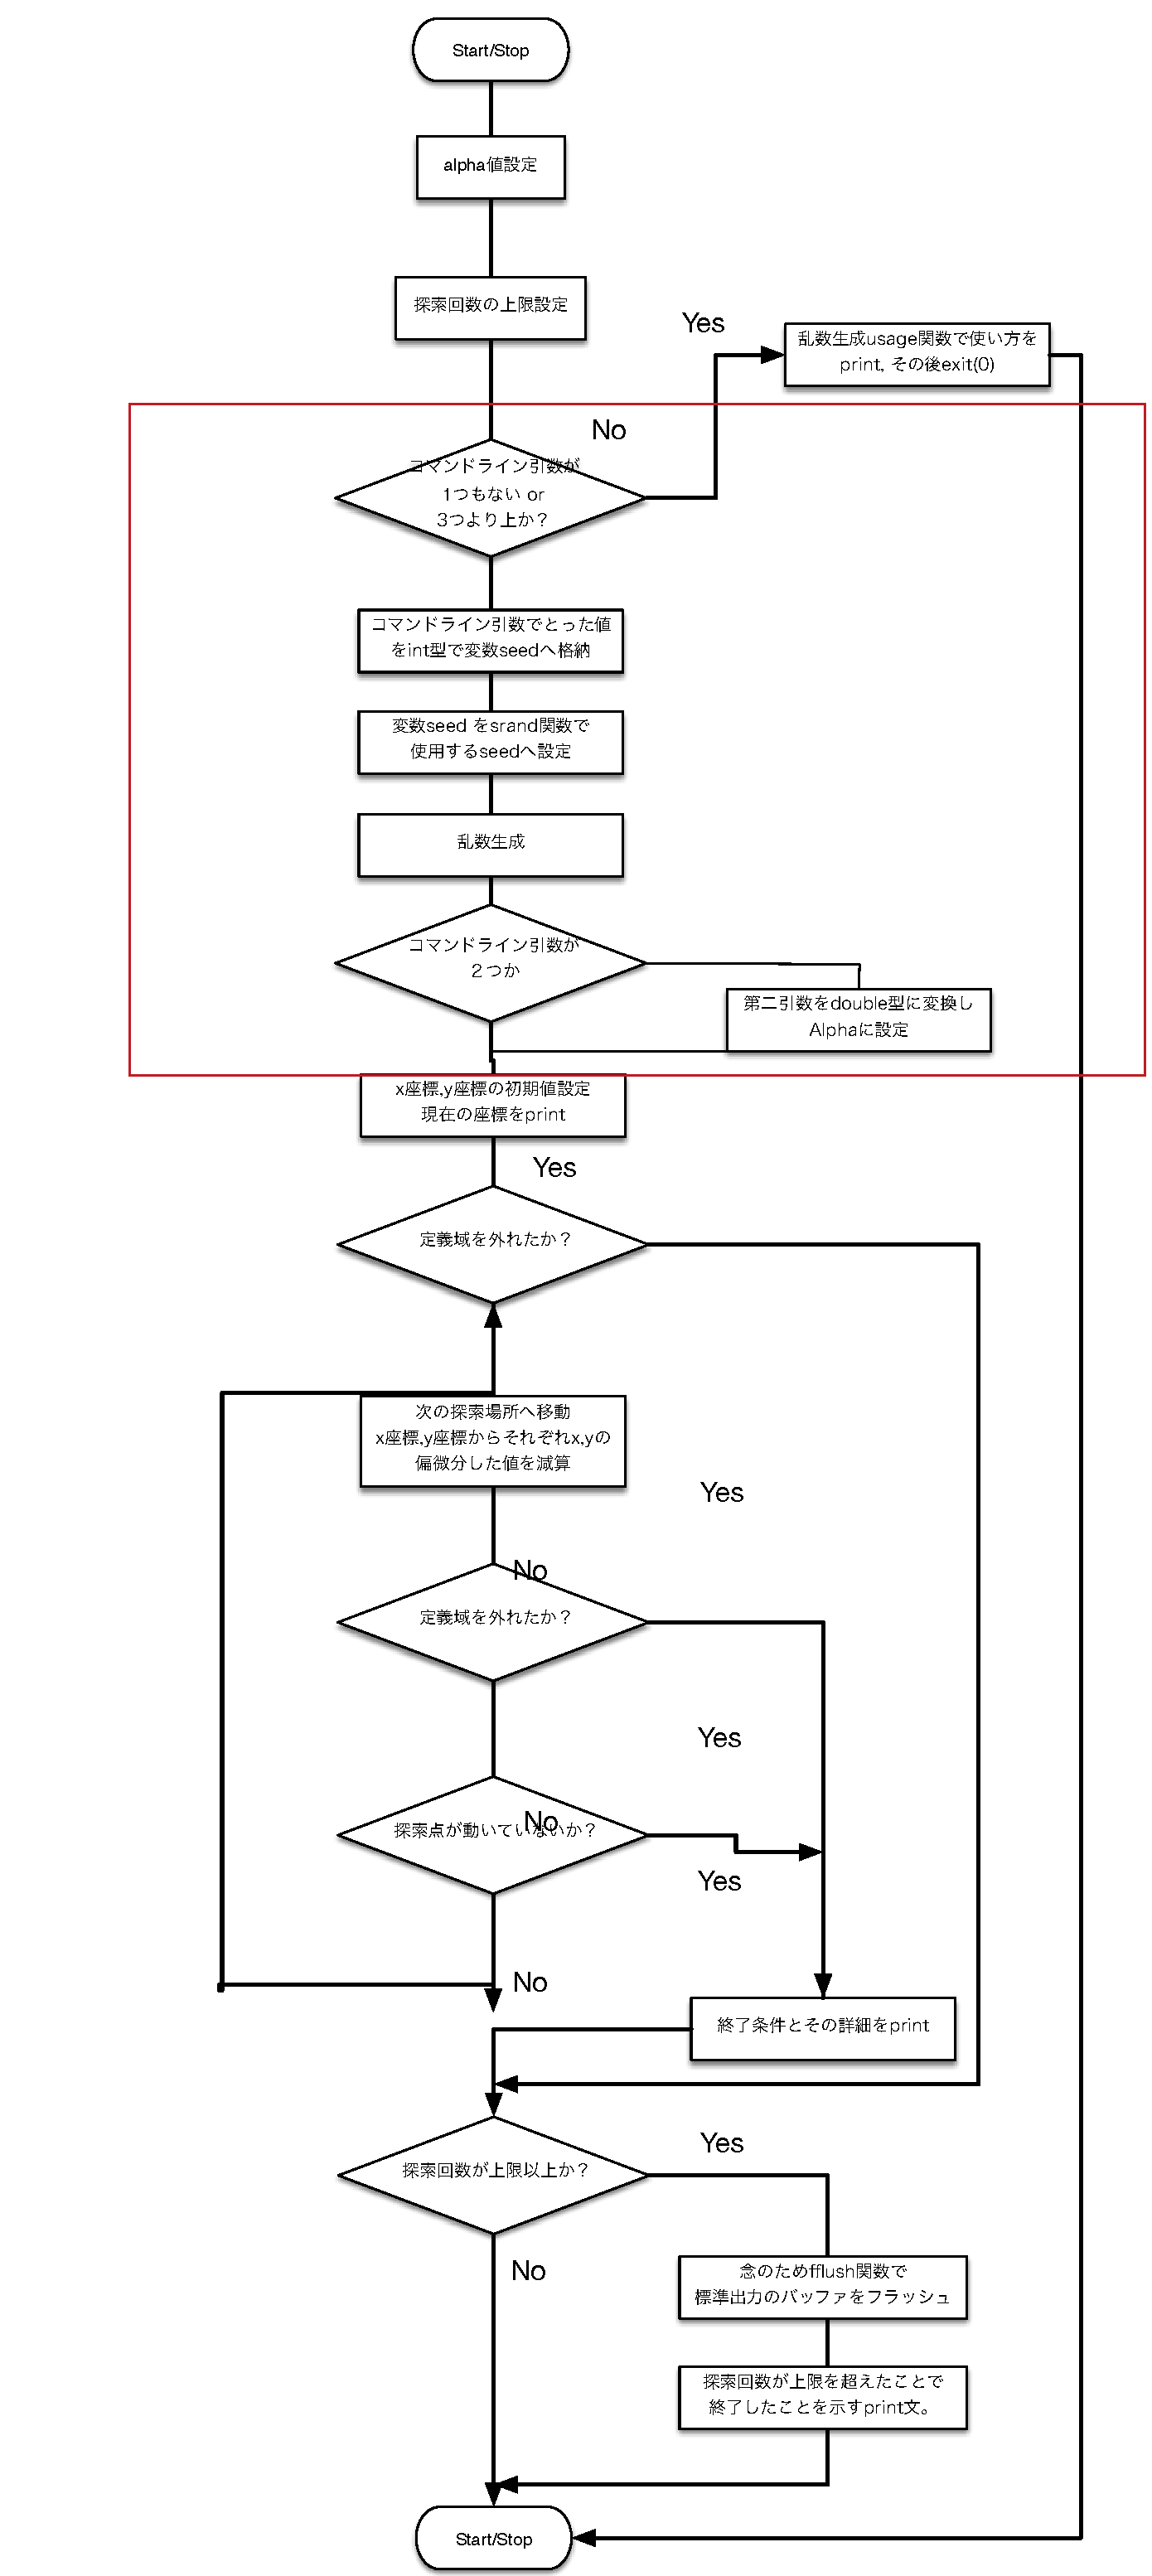
\includegraphics[width=0.5\textwidth]{figs/level2.3/flowchart3.pdf}
    \caption{level2.3フローチャート図}
\label{fig:flow23}
\end{figure}

\subsubsection{実験意図と観察方法}
最初に学習係数が探索に影響をあたえる物が何かを決定づけるため,seedを固定して学習係数Alphaのみ変更を行う.
実験では,最初に効率に着目しstepの回数を比較する.続いて,正確性を判断するためにシェルスクリプトを用いてモデル式の上に結果をplotし,確認を行った.

続いてseedがどのような影響を与えるかを観察する為,Alpha値を固定しseedを変更して観察を行った.内容はAlphaと同様に,step回数,及びモデル式との比較を行った.

\subsubsection{Alphaの変更実験}

まずAlphaの値を変更した場合,step数にどう変化があるかを実験する.
今回はシェルスクリプトを用いて自動化し,実験を行った.

スクリプトはrun\_ave.shを一部改変したrun\_ave\_alpha.shを利用した為,本レポートでは変更点を示す. (コード:\ref{code:runave})
尚ファイル名はaverageが入っているが,今回は平均値を取ってはおらず,複数回のループ処理の雛形として流用した.

\lstinputlisting[caption=run\_ave.shとrun\_ave\_alpha.shの差分,label=code:runave]{../steepestsearch2-3/shell_dif.log}

今回は結果を出力するテキストファイルを変数result\_file,gnuplotでの出力pdf名をpdf\_titleでそれぞれ設定している.
また,seed値を固定し,マジックナンバーを使用しない為に,変数seedに1000を設定している.

元のシェルスクリプトを参考にし,結果を書き出すテキストファイルがあれば削除するように変更した.
シェルスクリプト内でループをさせる場合,全要素を書き込んでループさせる事も考えられる.
しかし,今回は20パターン計測をする事を考えている.
この場合,学習係数Alphaの候補全要素を書き込むのは冗長と判断した.
故にwhile分で初期化しながら,配列roops\cite{shellq}を利用した.

今回は配列roopsに収納した変数20個分Alphaの初期値を0.01とし,0.1づつインクリメントしながら計測を行う.
計測をした結果をresult\_fileで設定したテキストファイルに書き込み,gnuplotを用いてpdf形式でグラフ化している.


このスクリプトを用いてグラフ化したものと,その際の実行結果を示す. (グラフ:図\ref{fig:runavesh} ,実行結果:コード\ref{code:runavealphalog})
\lstinputlisting[caption=run\_ave.shの実行結果,label=code:runavealphalog]{../steepestsearch2-3/run_ave_alpha.log}

\begin{figure}[H]
    \centering
    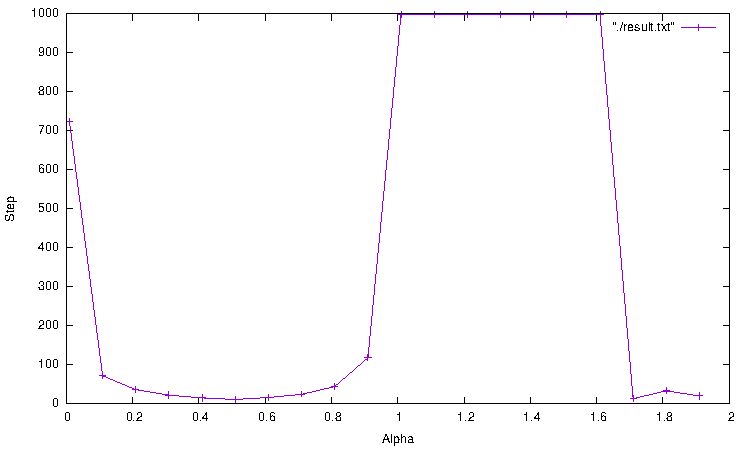
\includegraphics[width=0.5\textwidth]{figs/level2.3/alpha_ave.pdf}
    \caption{run\_ave.shの実行結果}
\label{fig:runavesh}
\end{figure}

step数という観点から見ると,2箇所で如実な減少が見られた.
しかし,今回のプログラムでは探索が正常に終了していない場合も含めている.
実行結果を見ると,FINISH 2で終了しているものは後半の3つしかなく,その中でも良い値はAlphaの値を1.71にした場合であった.

続いて実際に探索点がどのように動いたのか,精度の面から確認する.
まずは探索結果を可視化するために,スクリプトを生成した.
今回はtrans\_x\_vs\_func.shを参考に,run\_ave\_alpha.shを改良した.(ソースコード:\ref{transh})
\lstinputlisting[caption=trans\_alpha.shの変更点,label=transh]{../steepestsearch2-3/transalpha.log}

trans\_x\_vs\_func.shからは,cutコマンドで分割しテキストファイルにplotするデータを使用する部分のみに改良した.
大まかな処理はrun\_ave\_alpha.shと同様である.

20件のデータをまずplotすることを考え,ソースコード (\ref{transh})に一部加筆を行い,グラフ化を行った.
ソースコード (\ref{transh})との変更点は,gnuplotのplot呼び出しに対して,収集した全データを記述した点である.

全データをplotした結果を示す. (図:\ref{fig:alottrance})
また,プロンプトに表示された実行結果も併記する. (ソースコード:\ref{transhpro})
\lstinputlisting[caption=trans\_alpha.shの実行結果,label=transhpro]{../steepestsearch2-3/trance.log}

\begin{figure}[H]
    \centering
    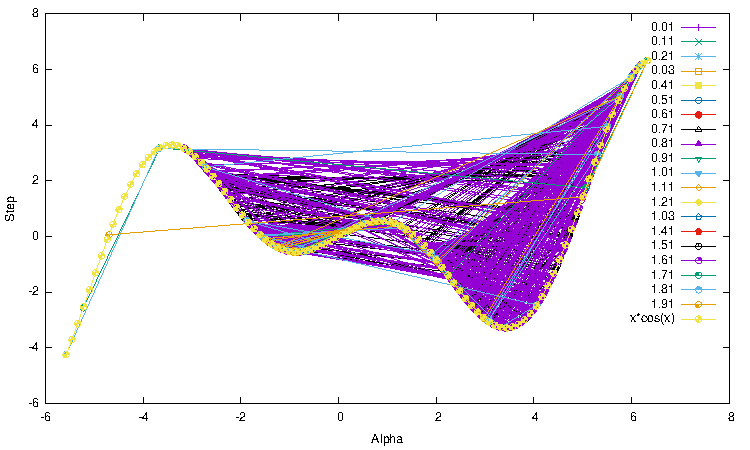
\includegraphics[width=0.5\textwidth]{figs/level2.3/alpha_ave_trans_alot.pdf}
    \caption{trans\_alpha.shを用いた全データの実行結果}
\label{fig:alottrance}
\end{figure}

データ件数が20件と多かった事と,動きがやや複雑なものがあり,動きを推測出来ないグラフとなってしまった.
そこで,先程step数が少なかった0.41,0.51,0.61,1.71,1.81,1.91とモデル式のみををplotし確認を行った.
\begin{figure}[H]
    \centering
    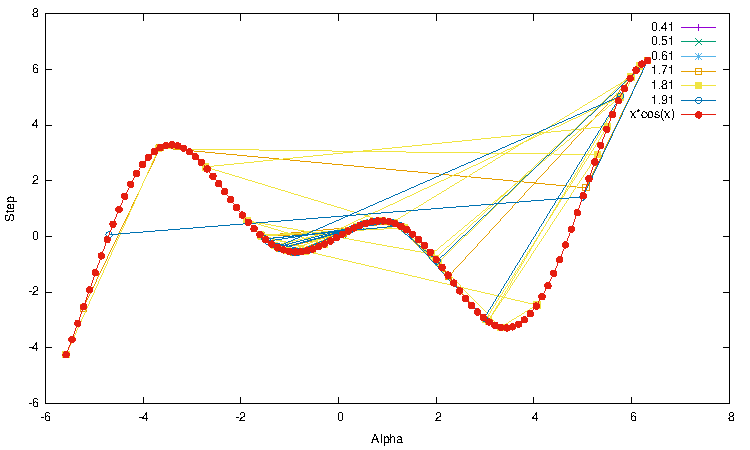
\includegraphics[width=0.5\textwidth]{figs/level2.3/alpha_ave_trans.pdf}
\caption{trans\_alpha.shを用いたデータの実行結果}
\label{fig:pickttrance}
\end{figure}

動きとしてはやや難があるが,1.81が比較的モデル式に沿って移動していると判断できる.
この事から,今回の結果では1.81が学習係数Alphaとしてふさわしいと考える.

\subsubsection{seedの変更実験}
続いてseedについて変更した結果どう変わるかを実験する.
今回は先程作成したrun\_ave\_alpha.shをseed用に変更した. (ソースコード:\ref{runseed})

\lstinputlisting[caption=run\_seed.shの変更点,label=runseed]{../steepestsearch2-3/runseed-dif.log}

今回はseed値の挙動を観察するため,初期値として1000を与え,ループのたびに1000インクリメントしていく方法に変更した.
実際にこのスクリプトを実行した結果得られたグラフを示す. (図:\ref{fig:seedave})

\begin{figure}[H]
    \centering
    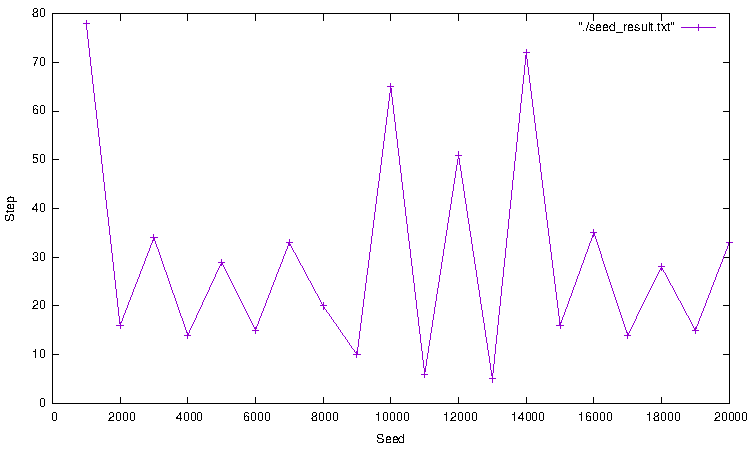
\includegraphics[width=0.5\textwidth]{figs/level2.3/seed_ave.pdf}
    \caption{run\_seed.shの実行結果}
\label{fig:seedave}
\end{figure}

このグラフから,seed値を1000区切りで変更するとstep値が上昇と下降を繰り返す結果が読み取れた.
この中では11000から13000ほどの間が尤も短いstep数であった為,ここに絞ってより細かく調査を行った.

調査用スクリプトとして範囲とループ数を変更したものを用意した. (ソースコード:\ref{runseedseed})
\lstinputlisting[caption=run\_seed\_seed.shの変更点,label=runseedseed]{../steepestsearch2-3/runseed-seed-dif.log}

今回は初期値を11000に設定し,500ずつ40回インクリメントを行い挙動を確認した.
このスクリプトを実行した結果,得られたグラフを示す.
\begin{figure}[H]
    \centering
    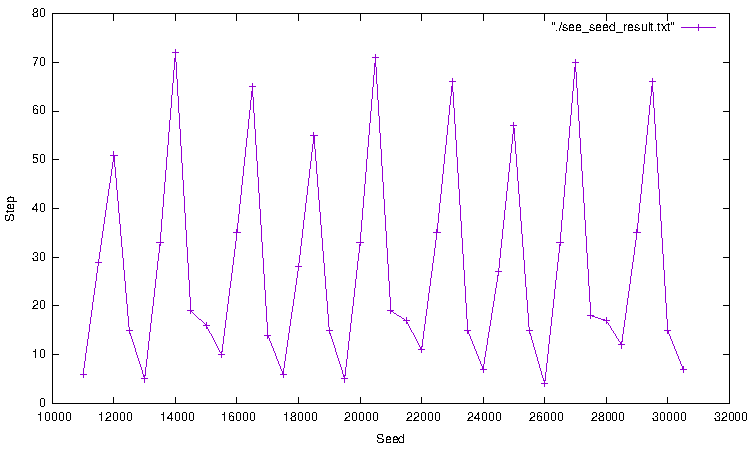
\includegraphics[width=0.5\textwidth]{figs/level2.3/see_seed_ave.pdf}
    \caption{run\_seed\_seed.shの実行結果}
\label{fig:seeseeddave}
\end{figure}

先程と同様に,STEP数が上昇と下降を繰り返しをしていることが確認出来た.
この結果から,Seed値26000が今回では有益なものであると考える.
尚このスクリプトは終了条件を特に設けていない為,得られた値が正しいものとは限らない.

では,今回seed値に応じてどのような探索経路を辿ったかを確認する.
今回はAlphaの実験同様にシェルスクリプトを用いて実験を行った.
利用したシェルスクリプトを示す. (ソースコード:\ref{trunseseed})

\lstinputlisting[caption=truns\_seed.sh,label=trunseseed]{../steepestsearch2-3/trans_seed.sh}

ほぼ構造はこれまで使ってきたシェルスクリプトと同じであり,今回は全てのデータではなく,ピックアップした幾つかの結果をグラフ化した.
このシェルスクリプトを実行した結果,出力されたグラフを示す. (グラフ:\ref{fig:seedtotal})

\begin{figure}[H]
    \centering
    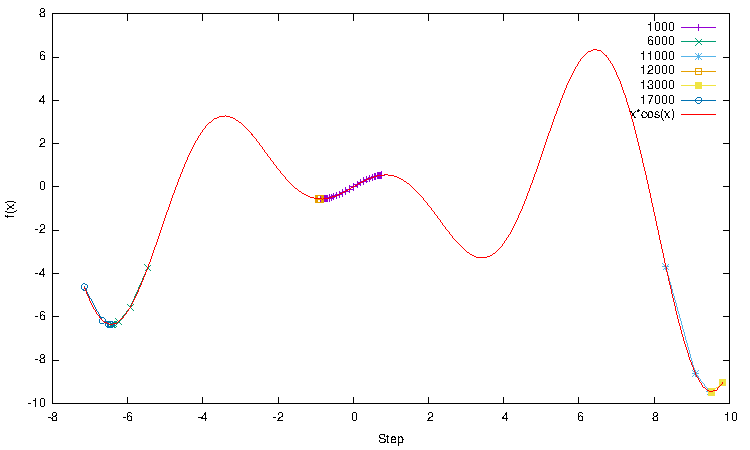
\includegraphics[width=0.8\textwidth]{figs/level2.3/seed_total.pdf}
    \caption{seed値による探索点の推移}
    \label{fig:seedtotal}
\end{figure}

結果から,seed値によっては,最終的に探索を終了する最小値に行き着いていない箇所があることが解る.
今回の範囲での最小値 (Stepが8から9の間)に収まったのは,Seed値11000と1300のみであった.

\subsubsection{考察}
今回の実行結果を踏まえると,Alphaの値を変えた場合,探索点がたどる経路が異なってくると推測できる.
Alphaの値が小さいほど,モデル式と類似した経路を辿り最小値に行き着く可能性が高い.ただし,Step数と探索自体の正確性では,やや疑問の残る結果となっしまった.
今回の結果では,極端にStep数が多い箇所,少ない箇所が観察できた.
従って,正確性を保ちつつStep数を少なくするには極めて細やかなチューニングが必要であるとも考える.

seed値の変更では,最終的に得られるf(x)の値が異なる事が読み取れた.
これは最急降下法のアルゴリズムが,一度最小値と思われる部分.
つまり切片の傾きが0の所に来てしまった場合,そこを最小値と認識し探索を終了することが原因していると考える.
今回のモデル式である$f=x*\cos(x)$は,この切片の傾きが0である箇所が複数ある.
その為,最急降下法を用いて正確な実験を行う場合初期探索位置を複数の場所に設定し,探索をすることが有効であると考える.
また,一度探索が終了する条件になった際に分岐させ,現在のx座標からある一定の数座標軸をずらし探索を行う.
その結果得られた解と分岐前の解を比較し,より良い結果を採用するなどの工夫が必要になってくると考えた.
